\documentclass[main.tex]{subfiles}
    \usepackage{amsmath}
    \usepackage{listings}
    \usepackage{amsfonts}
    \usepackage{amssymb}
    \usepackage{graphicx}
    \graphicspath{ {./img/} }
    
\begin{document}
\begin{enumerate}
	\item Man zeige direkt anhand der \( \epsilon \)-\( \delta \)-Definition die Stetigkeit der Funktion
	      \( f(x) = |x| \).
	      Wie kann man anhand der \( \epsilon \)-\(\delta \) Definition zeigen, dass die Signumsfunktion
	      \[ sign(x)= \begin{cases}
			      1  & x > 0, \\
			      0  & x = 0, \\
			      -1 & x < 0,
		      \end{cases}
	      \]
	      in \( x = 0 \) nicht stetig ist?

	      Lösung:
	      \[ \forall \xi \in \mathbb{R} | a - \xi | < \delta \Rightarrow | f(a) - f(\xi) | < \epsilon \]
	      \begin{enumerate}
		      \item \( f(x) = |x| \)

		            \( \forall \xi \in \mathbb{R} | a - \xi | < \delta \Rightarrow | f(a) - f(\xi) | < \epsilon \)

		            \( \delta = \epsilon \)

		            \( \forall \xi \in \mathbb{R} | a - \xi | < \delta \Rightarrow | f(0) - f(\xi) | = | 0 - \xi | < \epsilon \)
		      \item \( f(x) = sign(x), a = 0 \)

		            Die Bedingung muss für beliebig kleine \( \epsilon > 0 \) gelten, insbesondere für \( \epsilon < 1 \).

		            \( \delta = \epsilon \)

		            \( \forall \xi \in \mathbb{R} | 0 - \xi | < \delta \stackrel{\xi < 0}{\Rightarrow} | f(0) - f(\xi) | = | 0 + 1| \nleq \epsilon \)

		            \hspace{75pt} \( \stackrel{\xi > 0}{\Rightarrow} | f(0) - f(\xi) |  = | 0 - 1| \nleq \epsilon \)

		            \hspace{75pt} \( \stackrel{\xi = 0}{\Rightarrow} | f(0) - f(\xi) |  = | 0 - 0| < \epsilon \)

		            Die Aussage ist falsch für alle \( 0 < \epsilon < 1 \).
	      \end{enumerate}
	\item Man zeige
	      \[ x = e^{\ln{x}} \]
	      und leite durch beidseitiges Differenzieren eine Regel für
	      die Ableitung des Logarithmus her.

	      Lösung:
	      \begin{enumerate}
		      \item \( \frac{d}{dx} x = \frac{d}{dx} e^{\ln{x}} \)

		            \( 1 = (\frac{d}{dx} \ln{x}) \cdot e^{\ln{x}} \)

		            \( 1 = \frac{d}{dx}( \ln{x}) \cdot x  | \div x\)

		            \( \frac{1}{x} = \frac{d}{dx} \ln{x} \)
	      \end{enumerate}
	\item Bestimme die Ableitung der Funktion
	      \[ f(x) = -x + x \ln(x) \]
	      Was lässt sich daraus mithilfe der Gleichung
	      \( \int f'(x) dx = F(x) + C \) folgern?

	      Lösung:
	      \begin{enumerate}
		      \item \( f(x) = -x + x \ln(x) \)

		            \( f'(x) = -1 + x \cdot \frac{1}{x} + 1 \cdot \ln{x} \)

		            \( = -1 + 1 + \ln{x} \)

		            \( = \ln{x} \)

		      \item \( \int f'(x) dx = F(x) + C \)

		            \( \int ln(x) dx = [-x + x \ln{x}] = -x + x \ln{x} + C \)
	      \end{enumerate}
	\item Man leite mit Hilfe der Kettenregel die Ableitung von \( \frac{1}{ g(x) } \) und anschließend
	      mit der Produktregel die Ableitung von \( \frac{ f(x) }{ g(x) } \) her.

	      Lösung:
	      \begin{enumerate}
		      \item \( \frac{d}{dx} \frac{1}{g(x)} = \frac{d}{dx} g(x)^{-1} \)

		            \( = -1 \cdot g(x)^{-2} \cdot g'(x) \)

		            \( = - \frac{ g'(x) }{ g(x)^2 } \)
		      \item \( \frac{d}{dx} \frac{ f(x) }{ g(x) } = \frac{d}{dx} \Big( f(x) \cdot g(x)^{-1} \Big) \)

		            \( = f(x) \cdot g'(x) + f'(x) \cdot g(x) \)

		            \( = f(x) \cdot (- \frac{ g'(x) }{ g(x)^2 }) + f'(x) \cdot g(x)^{-1} \)

		            \( = \frac{- f(x) \cdot g'(x) }{ g(x)^2 } + \frac{f'(x) }{ g(x) } \)

		            \( = \frac{f'(x) \cdot g(x) }{ g(x)^2 } - \frac{f(x) \cdot g'(x) }{ g(x)^2 } \)

		            \( = \frac{f'(x) \cdot g(x) - f(x) \cdot g'(x) }{ g(x)^2 } \)
	      \end{enumerate}
	\item In der Vorlesung wurde die Ableitungsregel
	      \[ \frac{d}{dx} x^n = nx^{n-1} \]
	      direkt anhand der Definition der Ableitung gezeigt. Beweise diese Ableitungsregel
	      noch einmal mit vollständiger Induktion.

	      Lösung:
	      \begin{enumerate}
		      \item Induktionsvoraussetzung:
		            \( \frac{d}{dx} x^n = nx^{n-1} \)

		            Induktionsanfang: \( n = 0 \)

		            \( \frac{d}{dx} x^0 = \frac{d}{dx} 1 = 0 \)

		            \( 0 \cdot x^{0 - 1} = 0 \)

		            Induktionsschritt: \( n \rightarrow n + 1 \)

		            \( \frac{d}{dx} x^{n+1} = \frac{d}{dx} ( x^{n} \cdot x )  \)

		            \( = x^n \cdot \frac{d}{dx} x + \frac{d}{dx} x^n \cdot x \)

		            \( \stackrel{\text{nach Induktionsvoraussetzung}}{=} x^n \cdot 1 + nx^{n-1} \cdot x\)

		            \( = x^n + nx^n \)

		            \( = x^n(1 + n) \)
		            \( \square \)
	      \end{enumerate}
	\item Der Mittelwertsatz der Differentialrechnung lautet:

	      Die Funktion \( f \) sei im Intervall \( [a,b] \) stetig differenzierbar.
	      Dann existiert ein \( \xi \) mit
	      \[ f(b) - f(a)  = f'( \xi )( b - a ) \]
	      \begin{enumerate}
		      \item Was bedeutet der Satz anschaulich?
		      \item Beweise den Satz von Rolle:

		            Die Funktion \( f \) sei im Intervall \( [a,b] \) stetig differenzierbar und
		            es gelte \( f(a) = f(b) \). Dann besitzt der Graph von \( f \) zwischen
		            \( a \) und \( b \) mindestens einen Punkt mit waagrechter Tangente.
	      \end{enumerate}

	      Lösung:
	      \begin{enumerate}
		      \item
		      \item Nach dem Mittelwertsatz gilt:
		            \( \xi \in [a,b] \)

		            \( f(b) - f(a) = f'(\xi )(b-a) | \div(b-a) \)

		            \( \frac{f(b) - f(a)}{b - a} = f'( \xi ) \)

		            da \( f(a) = f(b) \)

		            \( \frac{0}{b - a} = f'( \xi ) \)

		            \( 0 = f'( \xi ) \)  \( \square \)
	      \end{enumerate}
	\item Wir betrachen die Funktion
	      \[ f(x) = \frac{ 3^3 + x^2 - 4 }{
			      4x^2 - 16
		      } \]
	      \begin{enumerate}
		      \item Man gebe den maximalen Definitionsbereich von \( f \) an.
		      \item Zeige die Identität
		            \[ f(x) - \frac{1}{4} = - \Bigg( f(-x) - \frac{1}{4} \Bigg)  \]

		            Was lässt sich daraus hinsichtlich der Symmetrie des Graphen von
		            \( f \) folgern?
		      \item Berechne die Schnittpunkte des Graphen von \( f \)  mit den Koordinatenachsen.
		      \item Bestimme alle Asymptoten von \( f \) und berechne die Schnittpunkte des
		            Graphen von \( f \)  mit der schiefen Asymptote.
		      \item Berechne die ersten beiden Ableitungen von \( f \).
		            Kontrolle:
		            \[ f'(x) = \frac{3}{4} \cdot x^2 \cdot \frac{ x^2 - 12 }{ (x^2 - 4)^2 } \]
		      \item Bestimme alle Extrempunkte.
		      \item Untersuche \( f \) auf Wendepunkte.
		      \item Zeichne den Graphen von \( f \) unter der Verwendung aller bisherigen Resultate.
	      \end{enumerate}

	      Lösung:
	      \begin{enumerate}
		      \item Definitionsbereich ist \( \mathbb{R} \)  ohne die Nullstellen des Nenners.

		            Nullstellen des Nenners:

		            \( 4x^2 - 16 = 0 | \div 4 \)

		            \( x^2 - 4 = 0 \)

		            \( x_{1,2} =- \frac{1}{2} \sqrt{\frac{1}{4} + 4} \)

		            \( x_1 = - \frac{1 + \sqrt{15}}{2} \)

		            \( x_2 = - \frac{1 - \sqrt{15} }{2} \)

		            \( D = \mathbb{R} \setminus \{ -\frac{1 + \sqrt{15}}{2}, -\frac{1 - \sqrt{15}}{2} \} \)
		      \item
		      \item Schnittpunkte mit der \( x \)-Achse sind die Nullstellen der Funktion. Der mit der
		            \( y \)-Achse kann durch einsetzen von \( f(0) \) ausgerechnet werden.

		            Nullstellen des Zählers:

		            \( 3x^3 + x^2 - 4 = 0 \)

		            Raten der Nullstelle \( x_1 = 1 \). Diese wird dann abgespaltet und so das
		            Polynom mit Polynomdivision um einen Grad reduziert.

		            \( (3x^3 + x^2 - 4)\div(x-1) = 3x^2 + 4x + 4 \)

		            \( x_{2,3} = \frac{-4 \pm \sqrt{16 - 4 \cdot 3 \cdot 4}}{2 \cdot 3} \)

		            \( x_{2,3} = - \frac{-4 \pm \sqrt{-32}}{6} \Rightarrow \)
		            Die beiden Nullstellen \( x_{2,3} \) sind irrational

		            Schnittpunkt mit der \( x \)-Achse: \( x_1 = 1 \)

		            Schnittpunkt mit der \( y \)-Achse:

		            \( f(0) = \frac{3\cdot0^3 + 0^2 -4}{4 \cdot 0^2 - 16} = \frac{-4}{-16} = \frac{1}{4} \)
		      \item Die Funktion hat eine schiefe Asymptote, da der Grad des Nenners um \( 1 \) grö0er ist, als der
		            des Zählers. Diese kann durch Polynomdivision ermittelt werden:

		            \( (3x^3 - x^2 - 4) \div (4x^2 - 16) = \frac{3}{4}x + \frac{1}{4} - \frac{12x}{4x^2 - 16} \)

		            Da der gebrochen rationale Teil des Polynoms für \( n \to \infty \) gegen \( 0 \) geht, ist
		            die Asymptote von \( f(x) \):

		            \( g(x) = \frac{3}{4}x + \frac{1}{4} \)
		      \item Um \( f(x) \) auf Wendepunkte zu untersuchen müssen die Nullstellen der \( 2. \) Ableitung ermittelt
		            werden.
			\item \begin{center}
			            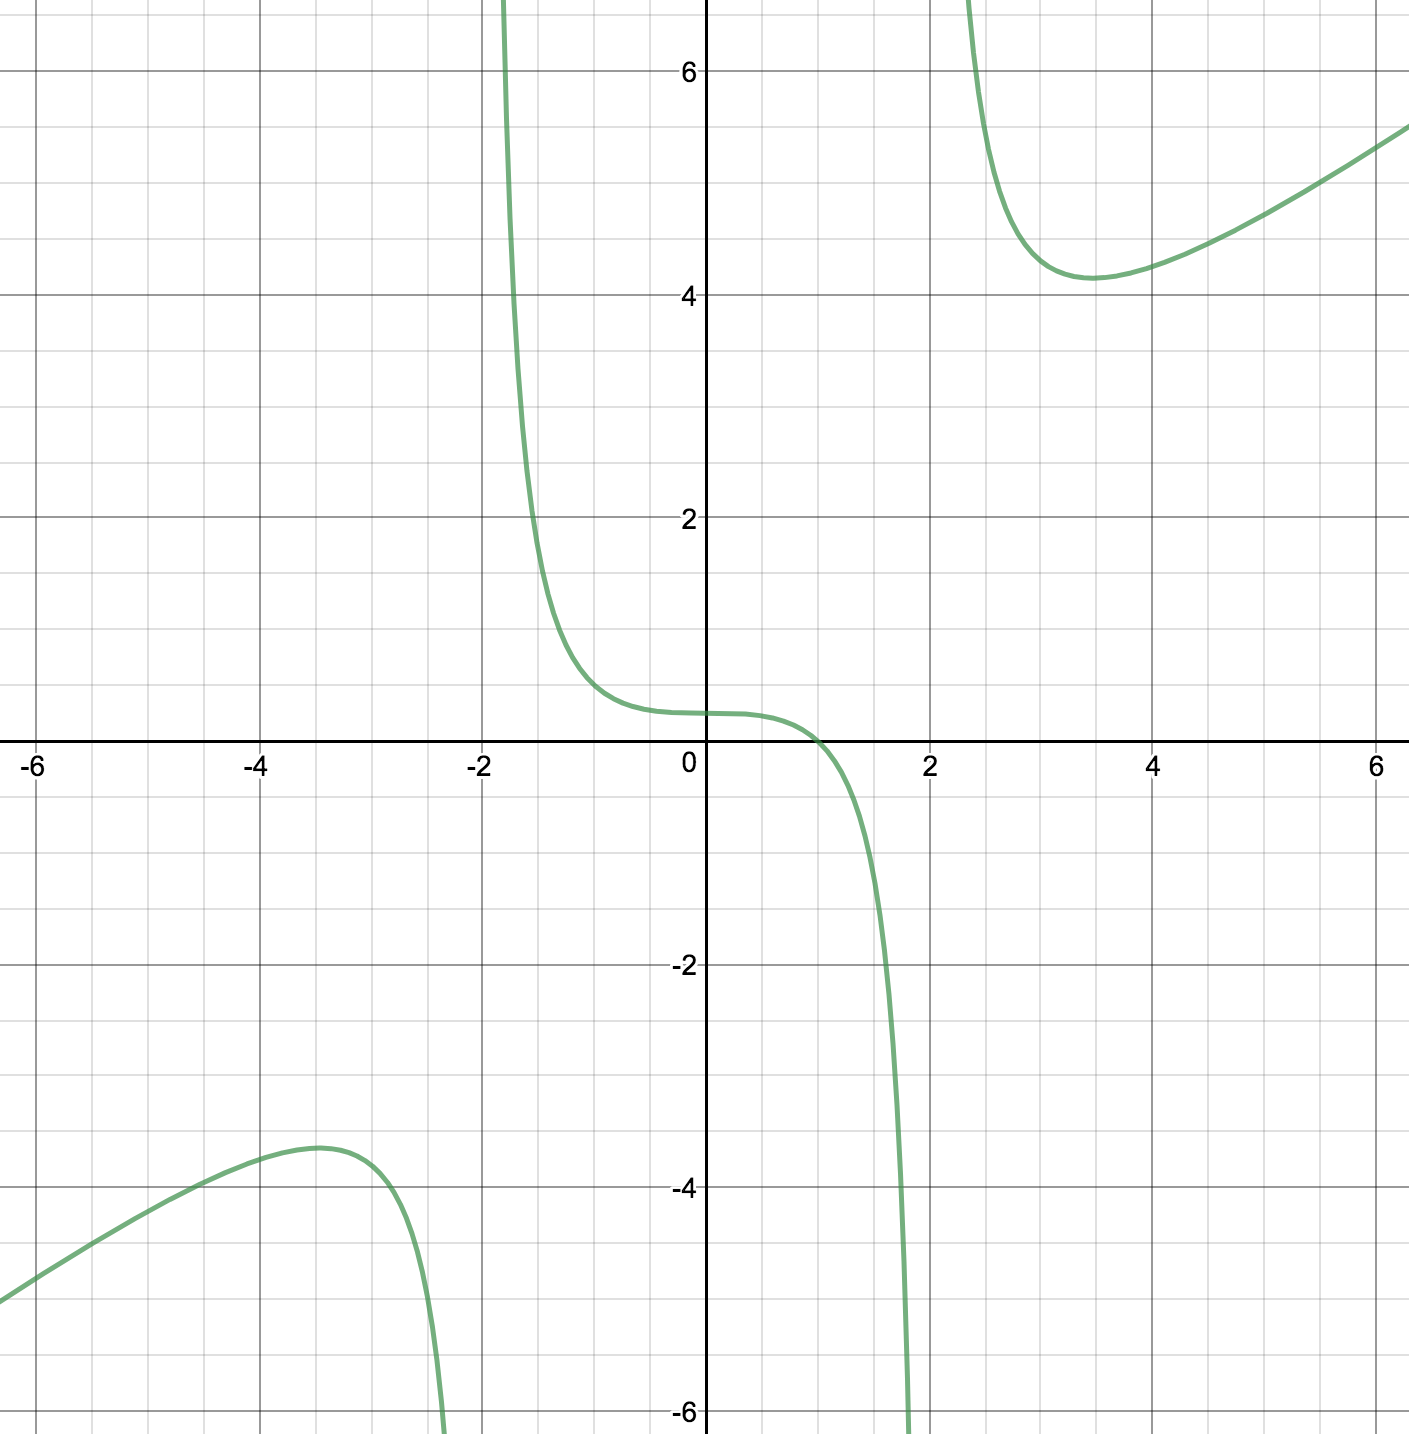
\includegraphics[scale=0.25]{analysisGraph}
		            \end{center}
	      \end{enumerate}
\end{enumerate}
\end{document}